%%
%% Copyright 2026 Elsevier Ltd
%%
%% This file is part of the 'Elsarticle Bundle'.
%% ---------------------------------------------
%%
%% It may be distributed under the conditions of the LaTeX Project Public
%% License, either version 1.2 of this license or (at your option) any
%% later version.  The latest version of this license is in
%%    http://www.latex-project.org/lppl.txt
%% and version 1.2 or later is part of all distributions of LaTeX
%% version 1999/12/01 or later.
%%
%% Template article for Elsevier's document class `elsarticle'
%% with numbered style bibliographic references
%% SP 2008/03/01

\documentclass[preprint,12pt, a4paper]{elsarticle}

\usepackage{amssymb}
\usepackage{amsmath}
\usepackage[T1]{fontenc}
\usepackage[utf8]{inputenc}
\usepackage[british]{babel}
\usepackage{booktabs}
\usepackage{xcolor}
\usepackage{tikz}
\usetikzlibrary{positioning,arrows.meta,fit,backgrounds}
\usepackage{hyperref}
\setlength{\parindent}{0pt}

%% Data that the authors still have to provide are marked in red
\newcommand{\todo}[1]{\textcolor{red}{[#1]}}
%% Sections still being planned are marked in blue
\newcommand{\plan}[1]{\textcolor{blue}{[Planned: #1]}}
\DeclareUrlCommand\file{\urlstyle{tt}}

\journal{SoftwareX}

\begin{document}

\begin{frontmatter}

\title{REC: A serverless tool to gamify quizzes and analyse students' answers offline}

\author[uca]{Lorena Gutiérrez-Madroñal\corref{cor1}}
\ead{lorena.gutierrez@uca.es}
\author[uca]{Rubén Baena-Pérez}
\author[uca]{José Miguel Mota-Macías}
\cortext[cor1]{Corresponding author.}

\address[uca]{Department of Computer Science and Engineering, School of Engineering, University of Cádiz, Avda.\ de la Universidad de Cádiz 10, 11519 Puerto Real, Cádiz, Spain}

\begin{abstract}
REC is a tool for gamifying quizzes that adapts to any course. Teachers import their Moodle XML questions into a browser-based studio and publish each contest encrypted on a static website, such as GitHub Pages, with no server or student accounts. Students play on any device, and each correct answer earns more points the sooner it is given. At the end, they send the teacher a ticket with a verification code and their answers in xAPI format. The studio builds rankings with a bonus for the final exam and, offline, analyses speed and accuracy to point out possible misconceptions before the next class.
\end{abstract}

\begin{keyword}
Gamification \sep Game-based learning \sep Student response systems \sep Learning analytics \sep xAPI
\end{keyword}

\end{frontmatter}

\section*{Required Metadata}
\label{sec:metadata}

\section*{Current code version}
\label{sec:codeversion}

\begin{table}[!h]
\small
\begin{tabular}{|l|p{5.6cm}|p{6.4cm}|}
\hline
\textbf{Nr.} & \textbf{Code metadata description} & \textbf{Please fill in this column} \\
\hline
C1 & Current code version & v1.0.0 (\url{https://doi.org/10.5281/zenodo.23594648}) \\
\hline
C2 & Permanent GitHub link to code/repository used for this code version & \url{https://github.com/lorenagmad/REC} \\
\hline
C3 & Legal Code License & AGPL-3.0-or-later \\
\hline
C4 & Code versioning system used & git \\
\hline
C5 & Software code languages, tools, and services used & JavaScript (ECMAScript 2020), HTML5, CSS3; Web Crypto, IndexedDB and Web Audio APIs; no third-party libraries \\
\hline
C6 & Compilation requirements, operating environments \& dependencies & A current web browser (Chrome, Edge, Firefox or Safari) on a computer, tablet or phone; any static web host with HTTPS, such as GitHub Pages, to publish contests \\
\hline
C7 & If available Link to developer documentation/manual & \url{https://github.com/lorenagmad/REC/blob/main/docs/GUIDE.md} \\
\hline
C8 & Support email for questions & \href{mailto:lorena.gutierrez@uca.es}{lorena.gutierrez@uca.es} \\
\hline
\end{tabular}
\caption{Code metadata (mandatory)}
\label{tab:codemetadata}
\end{table}

%% ============================================================================
\section{Motivation and significance}
\label{sec:motivation}

Game-based student response systems such as Kahoot! have become common in higher education, where they are used to increase participation and to give students immediate feedback~\cite{wang2020}. At the University of Cádiz, a teaching-innovation project running since the 2017/18 academic year in the course \emph{Herramientas Multimedia y Animación}, now \emph{Animación y Nuevas Tecnologías en Publicidad}, scores the quizzes held after each lecture by correctness and response speed, and the resulting rankings reward students in the final exam~\cite{gutierrez2018}. Encouraging participation is therefore no longer the main challenge. What teachers still lack is an analysis of what each student has actually learnt, built from their answers during the quiz and kept in the teacher's hands rather than the provider's.

The tool presented here grew out of this practice. In late 2019, the free plan of Kahoot! for higher education was limited to 50 players per live game, and in 2021 to 10~\cite{kahoot2019,kahoot2021}, which made it unusable in the course \emph{Fundamentos Técnicos en la Publicidad Digital}, with about 150 students. Moving the quizzes to Moodle, the institutional learning management system, solved the problem of scale but not that of scoring, because Moodle quizzes do not rank students by correctness and response speed. Each quiz had to be downloaded, filtered and scored in a spreadsheet, and the ranking then published in the virtual campus by hand. This took 15 to 30 minutes per quiz, that is, 3 to 6.5 hours per semester for the 13 quizzes of the animation course.

Commercial game-based response systems such as Kahoot!~\cite{kahoot}, Wayground (formerly Quizizz)~\cite{wayground}, Socrative~\cite{socrative}, Blooket~\cite{blooket}, Gimkit~\cite{gimkit} and Mentimeter~\cite{mentimeter} let students join without an account, and several of them award points for speed. However, they store students' answers on the provider's servers, and their free plans limit the number of players or the export of results (Table~\ref{tab:comparison}). The Moodle quiz~\cite{moodlequiz} keeps the data within the institution and imports Moodle XML, but it requires student accounts and does not score speed. Open-source alternatives such as ClassQuiz~\cite{classquiz} and QuizDock~\cite{quizdock} can be self-hosted, but they need a server with a database. Response times also carry information about learning: answers that reflect misconceptions tend to be given faster than correct ones~\cite{heckler2015}, and in gamified quizzes the response time of wrong answers helps to tell guesses from weak recall~\cite{liang2024}. According to their documentation, none of these tools combines speed and correctness in its analysis of students' answers.

\begin{table}[!htb]
\centering
\caption{Comparison with related tools, according to their documentation (October 2026). Speed: points depend on response time; Static: runs as static files, with no application server or database; No cloud: answers are not stored on the provider's servers; Moodle XML: imports Moodle XML questions; Times: exports each student's response time per question; Speed$\times$acc.: built-in analysis combining speed and correctness; Retention: built-in analysis across sessions; xAPI: exports xAPI statements; 150 free: a free game for about 150 students. \checkmark{} yes; $\circ$ partial; $\times$ no; ? not documented.}
\label{tab:comparison}\vspace{3pt}
\small\setlength{\tabcolsep}{3pt}
\resizebox{\textwidth}{!}{%
\begin{tabular}{lccccccccc}
\toprule
Tool & Speed & Static & No cloud & Moodle XML & Times & Speed$\times$acc. & Retention & xAPI & 150 free \\
\midrule
REC & \checkmark & \checkmark & \checkmark & \checkmark & \checkmark & \checkmark & \checkmark & \checkmark & \checkmark \\
Kahoot!~\cite{kahoot} & \checkmark & $\times$ & $\times$ & $\times$ & $\circ$\textsuperscript{a} & $\times$ & $\circ$\textsuperscript{a} & ? & $\times$ \\
Wayground~\cite{wayground} & $\circ$\textsuperscript{a} & $\times$ & $\times$ & ? & $\circ$ & $\times$ & ? & ? & $\times$ \\
Socrative~\cite{socrative} & $\times$ & $\times$ & $\times$ & $\times$ & $\times$ & $\times$ & ? & ? & $\times$ \\
Moodle quiz~\cite{moodlequiz} & $\times$ & $\times$ & $\circ$\textsuperscript{b} & \checkmark & $\times$ & $\times$ & $\times$ & $\times$ & \checkmark \\
Blooket~\cite{blooket} & \checkmark & $\times$ & $\times$ & $\times$ & $\circ$\textsuperscript{c} & $\times$ & ? & ? & $\times$ \\
Gimkit~\cite{gimkit} & $\times$ & $\times$ & $\times$ & $\times$ & $\times$ & $\times$ & $\times$ & ? & \checkmark \\
Mentimeter~\cite{mentimeter} & \checkmark & $\times$ & $\times$ & ? & ? & $\times$ & ? & ? & $\circ$ \\
\bottomrule
\end{tabular}}

\vspace{2pt}{\footnotesize \textsuperscript{a}~Paid plans only. \textsuperscript{b}~Stored on the institution's server. \textsuperscript{c}~Average time per question only.}
\end{table}

REC was developed under three requirements: (i)~to reuse the questions teachers already have in Moodle, through the import of Moodle XML; (ii)~to run in any browser without student accounts or servers, with contests published encrypted on a static website and opened with a password; and (iii)~to give the teacher an analysis of each student's answers, combining speed and correctness, with the data held by the teacher. The teacher prepares the contests in the studio and publishes them encrypted. After the lecture, all students play at the same time, each on their own device (phone, tablet or laptop), with the password given in class; nothing is projected during the quiz. At the end, each student obtains a ticket with a verification code, with which the studio detects tickets that have been modified, and a results file in xAPI format~\cite{xapi}, which they submit through the virtual campus. The teacher then verifies the tickets, builds and publishes the ranking, and analyses the results. The same tool supports graded continuous assessment, with rankings that reward students in the final exam, and ungraded diagnostic quizzes held before a topic is taught, which also record attendance.

%% ============================================================================
\section{Software description}
\label{sec:description}

REC~1.0.0~\cite{rec} is a web application written in JavaScript (ECMAScript 2020), HTML5 and CSS3. It uses no third-party libraries or frameworks, only standard browser interfaces (Web Crypto, IndexedDB, Web Audio, Fetch and the DOM), so that teachers need neither to program nor to install anything. The interface is available in Spanish and English. REC was developed by the authors with the assistance of a generative artificial-intelligence model (Claude, Anthropic): the authors specified the requirements, took the design decisions, and reviewed and tested the code.

\subsection{Software architecture}
\label{sec:architecture}

REC consists of two self-contained files, each holding its own HTML, CSS and JavaScript (Figure~\ref{fig:flow}). The \emph{studio} (\file{studio.html}) is used by the teacher, and the \emph{studio floor} (\file{index.html}) by the students. A REC site is simply a folder with these two files and a \file{contests} subfolder, which any static web host with HTTPS can serve; a ready-to-upload kit and step-by-step guides for GitHub Pages are included in the repository.

The studio keeps the teacher's project (course, question bank, contests and passwords) in the browser's IndexedDB and can save it to, or load it from, a JSON file. To publish, it encrypts each contest separately with AES-GCM (256-bit key derived from the contest password with PBKDF2-SHA-256, 300,000 iterations) and generates a ZIP package with the encrypted contests and a plain index of titles and settings. Unencrypted questions therefore never leave the teacher's computer; the project file, which is not encrypted, is meant to stay there too, as the studio warns. The studio floor downloads the index, decrypts the contest the student chooses with the password given in class, runs it, and produces the results locally. Sounds are synthesised with the Web Audio API, so the site contains no audio files.

\begin{figure}[!htb]
\centering
\resizebox{\textwidth}{!}{%
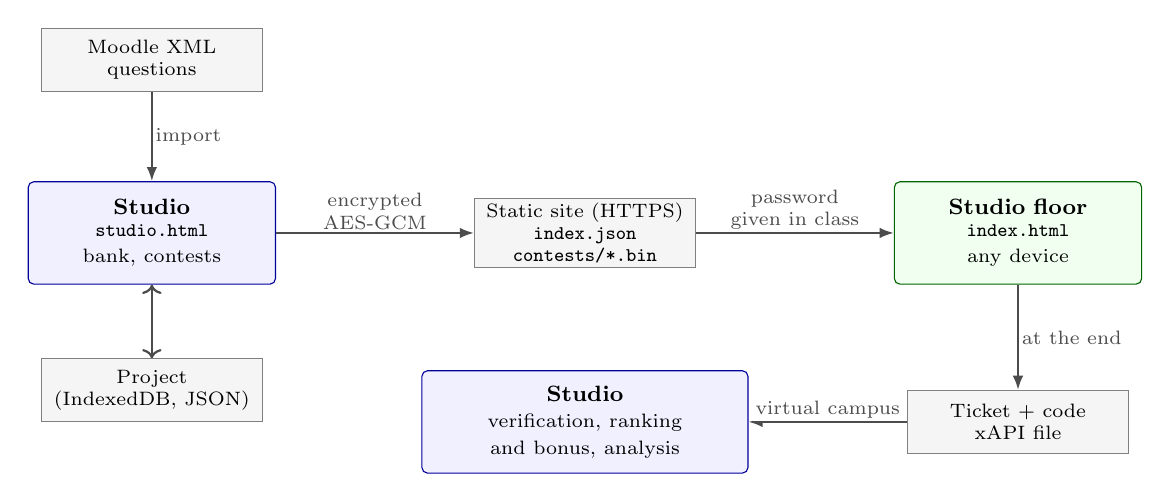
\begin{tikzpicture}[x=1mm, y=1mm, font=\footnotesize,
  tea/.style={draw=blue!60!black, fill=blue!6, rounded corners=2pt, align=center, minimum height=13mm, text width=30mm, inner sep=2pt},
  stu/.style={draw=green!40!black, fill=green!6, rounded corners=2pt, align=center, minimum height=13mm, text width=30mm, inner sep=2pt},
  dat/.style={draw=black!50, fill=black!4, align=center, minimum height=8mm, text width=27mm, inner sep=1.5pt, font=\scriptsize},
  arr/.style={-{Latex[length=1.8mm]}, thick, black!70},
  lab/.style={font=\scriptsize, align=center, fill=white, inner sep=1pt}]
  \node[dat] (moodle) at (0,22) {Moodle XML\\ questions};
  \node[tea] (studio) at (0,0) {\textbf{Studio}\\ \scriptsize\texttt{studio.html}\\ bank, contests};
  \node[dat] (project) at (0,-20) {Project\\ (IndexedDB, JSON)};
  \node[dat] (site) at (55,0) {Static site (HTTPS)\\ \texttt{index.json}\\ \texttt{contests/*.bin}};
  \node[stu] (floor) at (110,0) {\textbf{Studio floor}\\ \scriptsize\texttt{index.html}\\ any device};
  \node[dat] (ticket) at (110,-24) {Ticket + code\\ xAPI file};
  \node[tea, text width=40mm] (results) at (55,-24) {\textbf{Studio}\\ \scriptsize verification, ranking and bonus, analysis};
  \draw[arr] (moodle) -- node[lab, right]{import} (studio);
  \draw[arr, <->] (studio) -- (project);
  \draw[arr] (studio) -- node[lab, above]{encrypted\\ AES-GCM} (site);
  \draw[arr] (site) -- node[lab, above]{password\\ given in class} (floor);
  \draw[arr] (floor) -- node[lab, right]{at the end} (ticket);
  \draw[arr] (ticket) -- node[lab, above]{virtual campus} (results);
\end{tikzpicture}}
\caption{Architecture and workflow of REC. The teacher's studio (blue) publishes encrypted contests on a static site; students play on the studio floor (green) and send their tickets, which the studio verifies and analyses. Unencrypted questions stay on the teacher's computer.}
\label{fig:flow}
\end{figure}

\subsection{Software functionalities}
\label{sec:functionalities}

\paragraph{Question bank} Questions are imported from Moodle XML, with their images, videos and feedback, so that teachers can reuse the quizzes they already have, or created in the studio. Six types are supported: multiple choice with one or several correct answers, true/false, matching, ordering, short answer with wildcards, and point on an image, whose correct zones are drawn on the image. Images are compressed on import, videos are linked from YouTube or Vimeo, and questions are organised by topic.

\paragraph{Contests} A contest is a selection of questions with its own password, section, time per question type and score range, and the phrases of Cam, the host (Figure~\ref{fig:contest}). Contests are grouped by section on the home board, so that each course can arrange them by blocks or topics. Global tests for a block are generated automatically from its contests and topics, and each contest can also be offered in practice mode, without scoring, for self-study.

\begin{figure}[!htb]
\centering
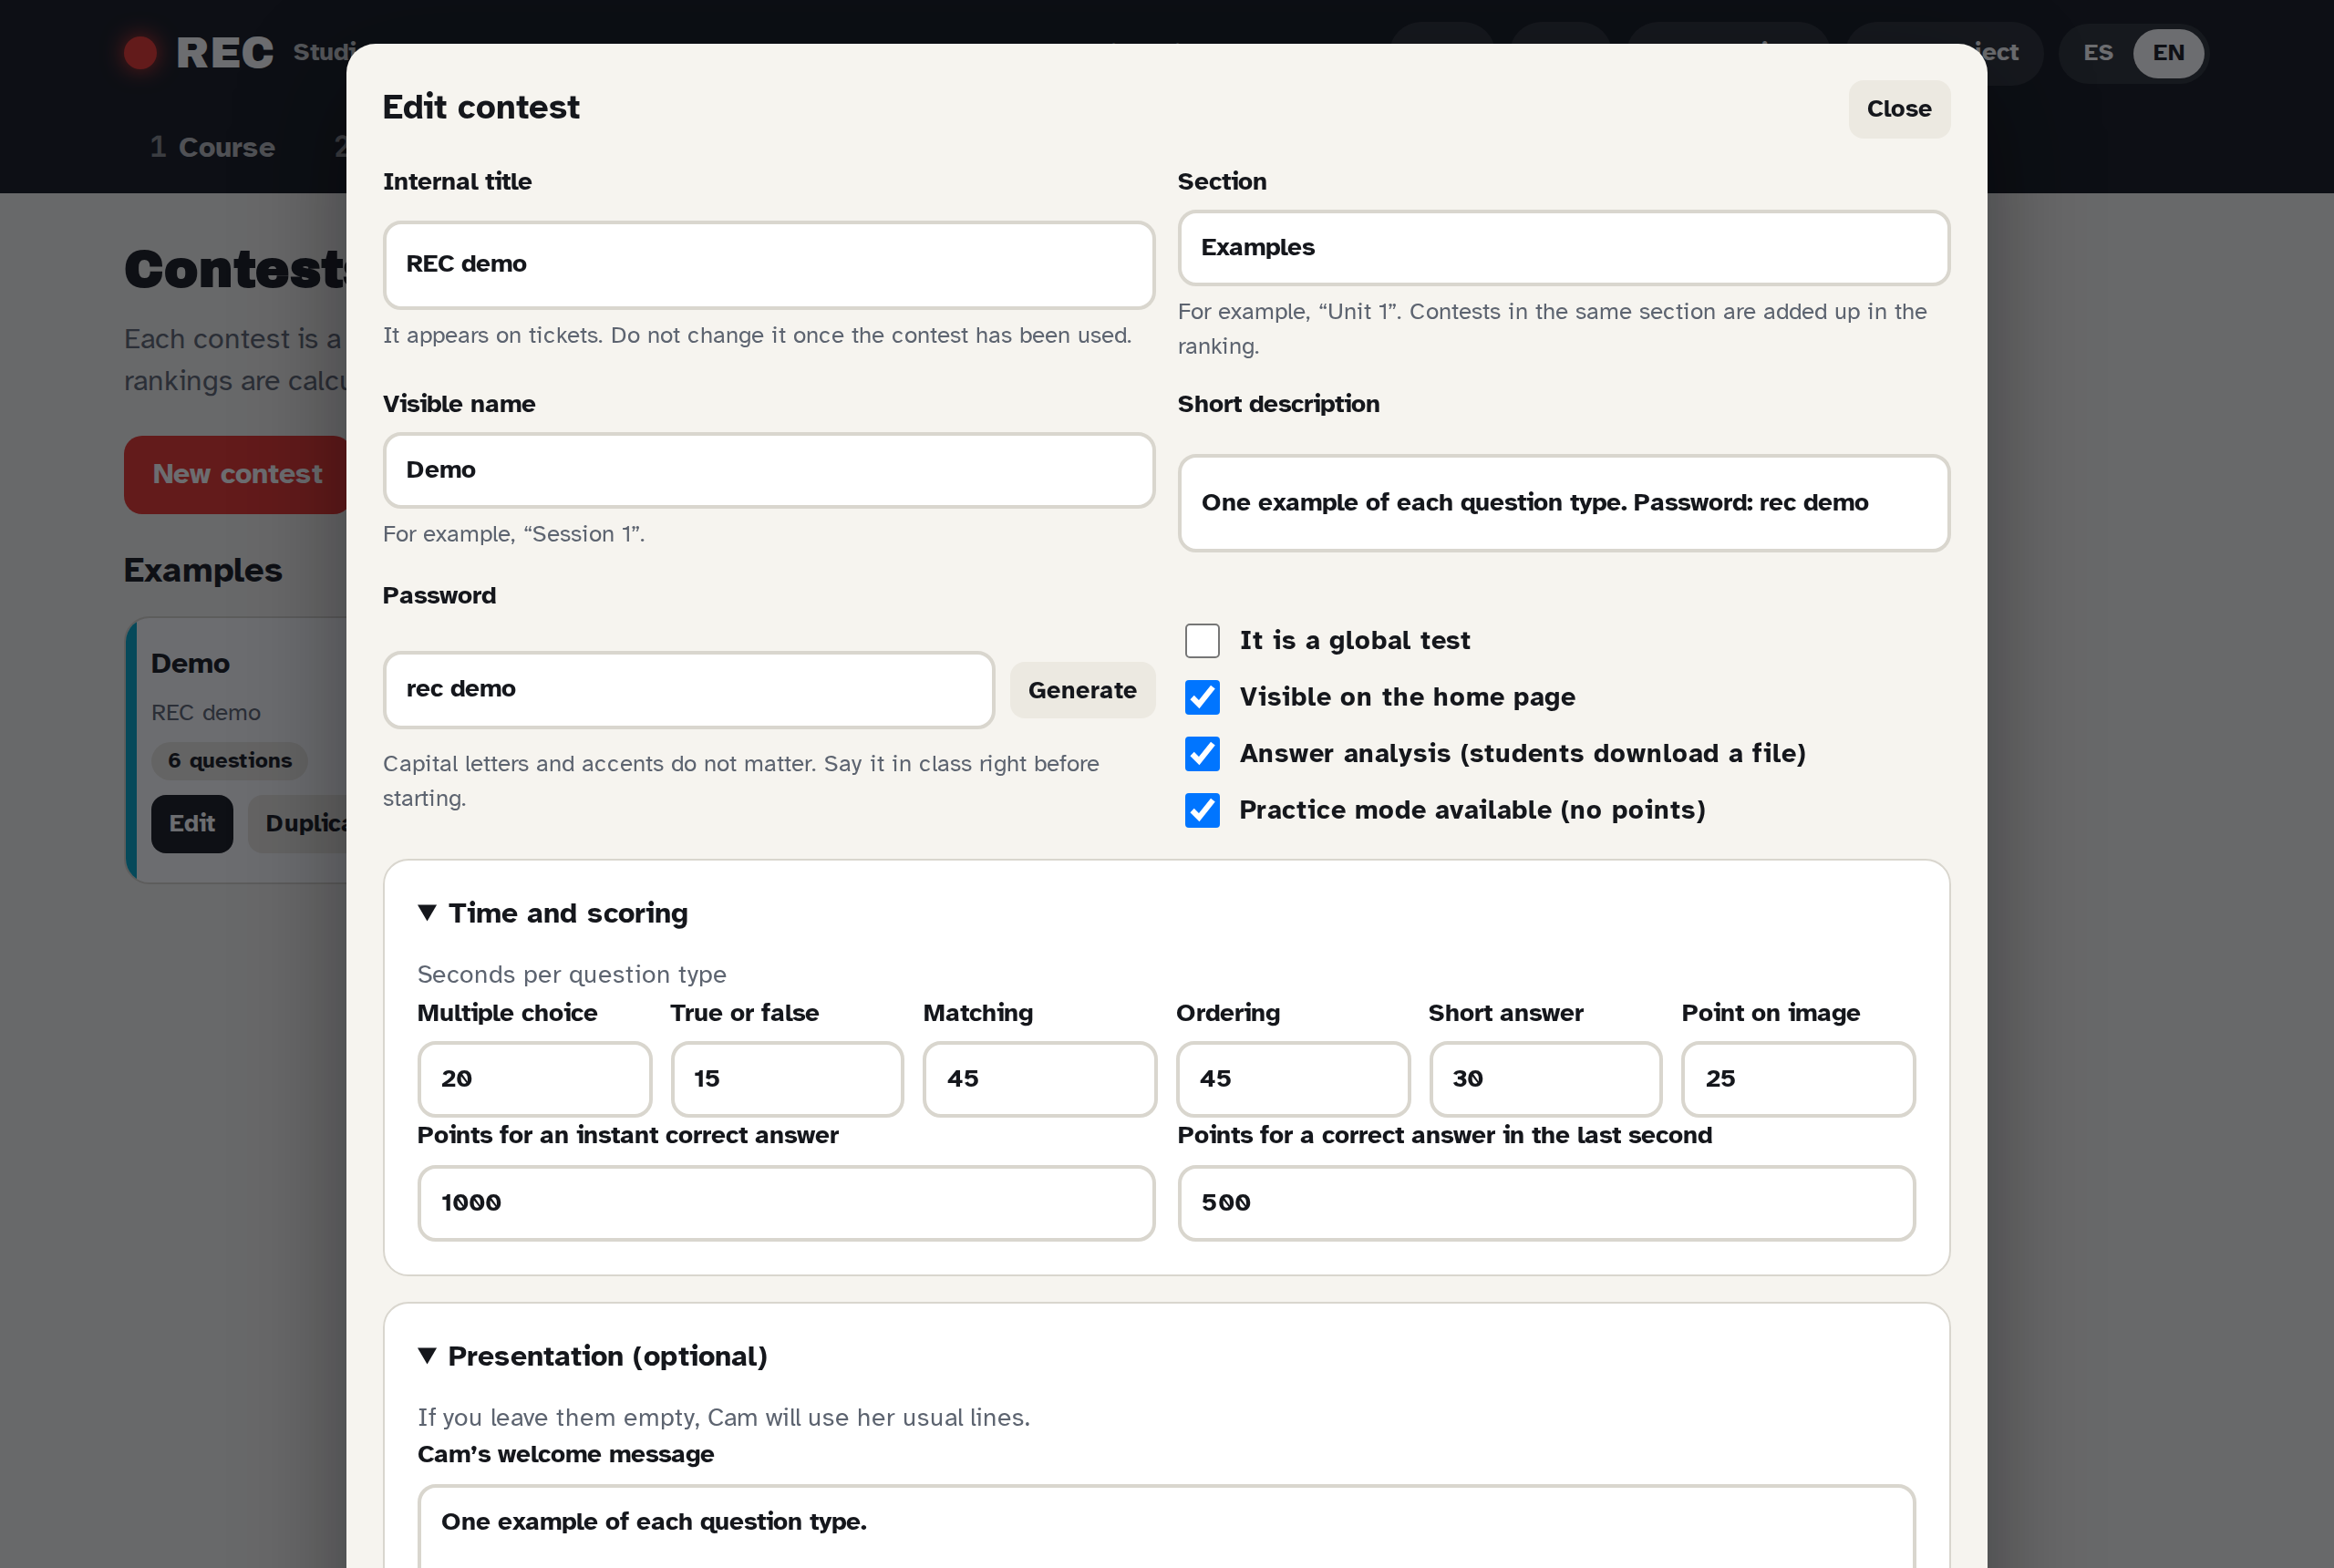
\includegraphics[width=0.85\textwidth]{figures/23c-studio-contest-settings.png}
\caption{Editing a contest in the studio: password, section, practice mode, answer analysis, time per question type and score range.}
\label{fig:contest}
\end{figure}

\paragraph{Playing} The studio floor presents the questions in random order with a countdown and game-show effects (Figure~\ref{fig:floor}). A correct answer earns from the maximum down to the minimum score (1,000 to 500 by default) depending on the time used, and partly correct answers earn a proportional share. The minimum keeps a reward for students who answer correctly but slowly, since time pressure is one of the drawbacks reported for game-based response systems~\cite{wang2020}; streaks are celebrated by the host but add no points. Students who need more time receive a personal code, linked to their identity, that extends the time limits by a given percentage. For accessibility, students can enlarge the text, switch to high contrast and reduce animations, and the browser remembers these choices.

\begin{figure}[!htb]
\centering
\begin{minipage}[c]{0.6\textwidth}\centering
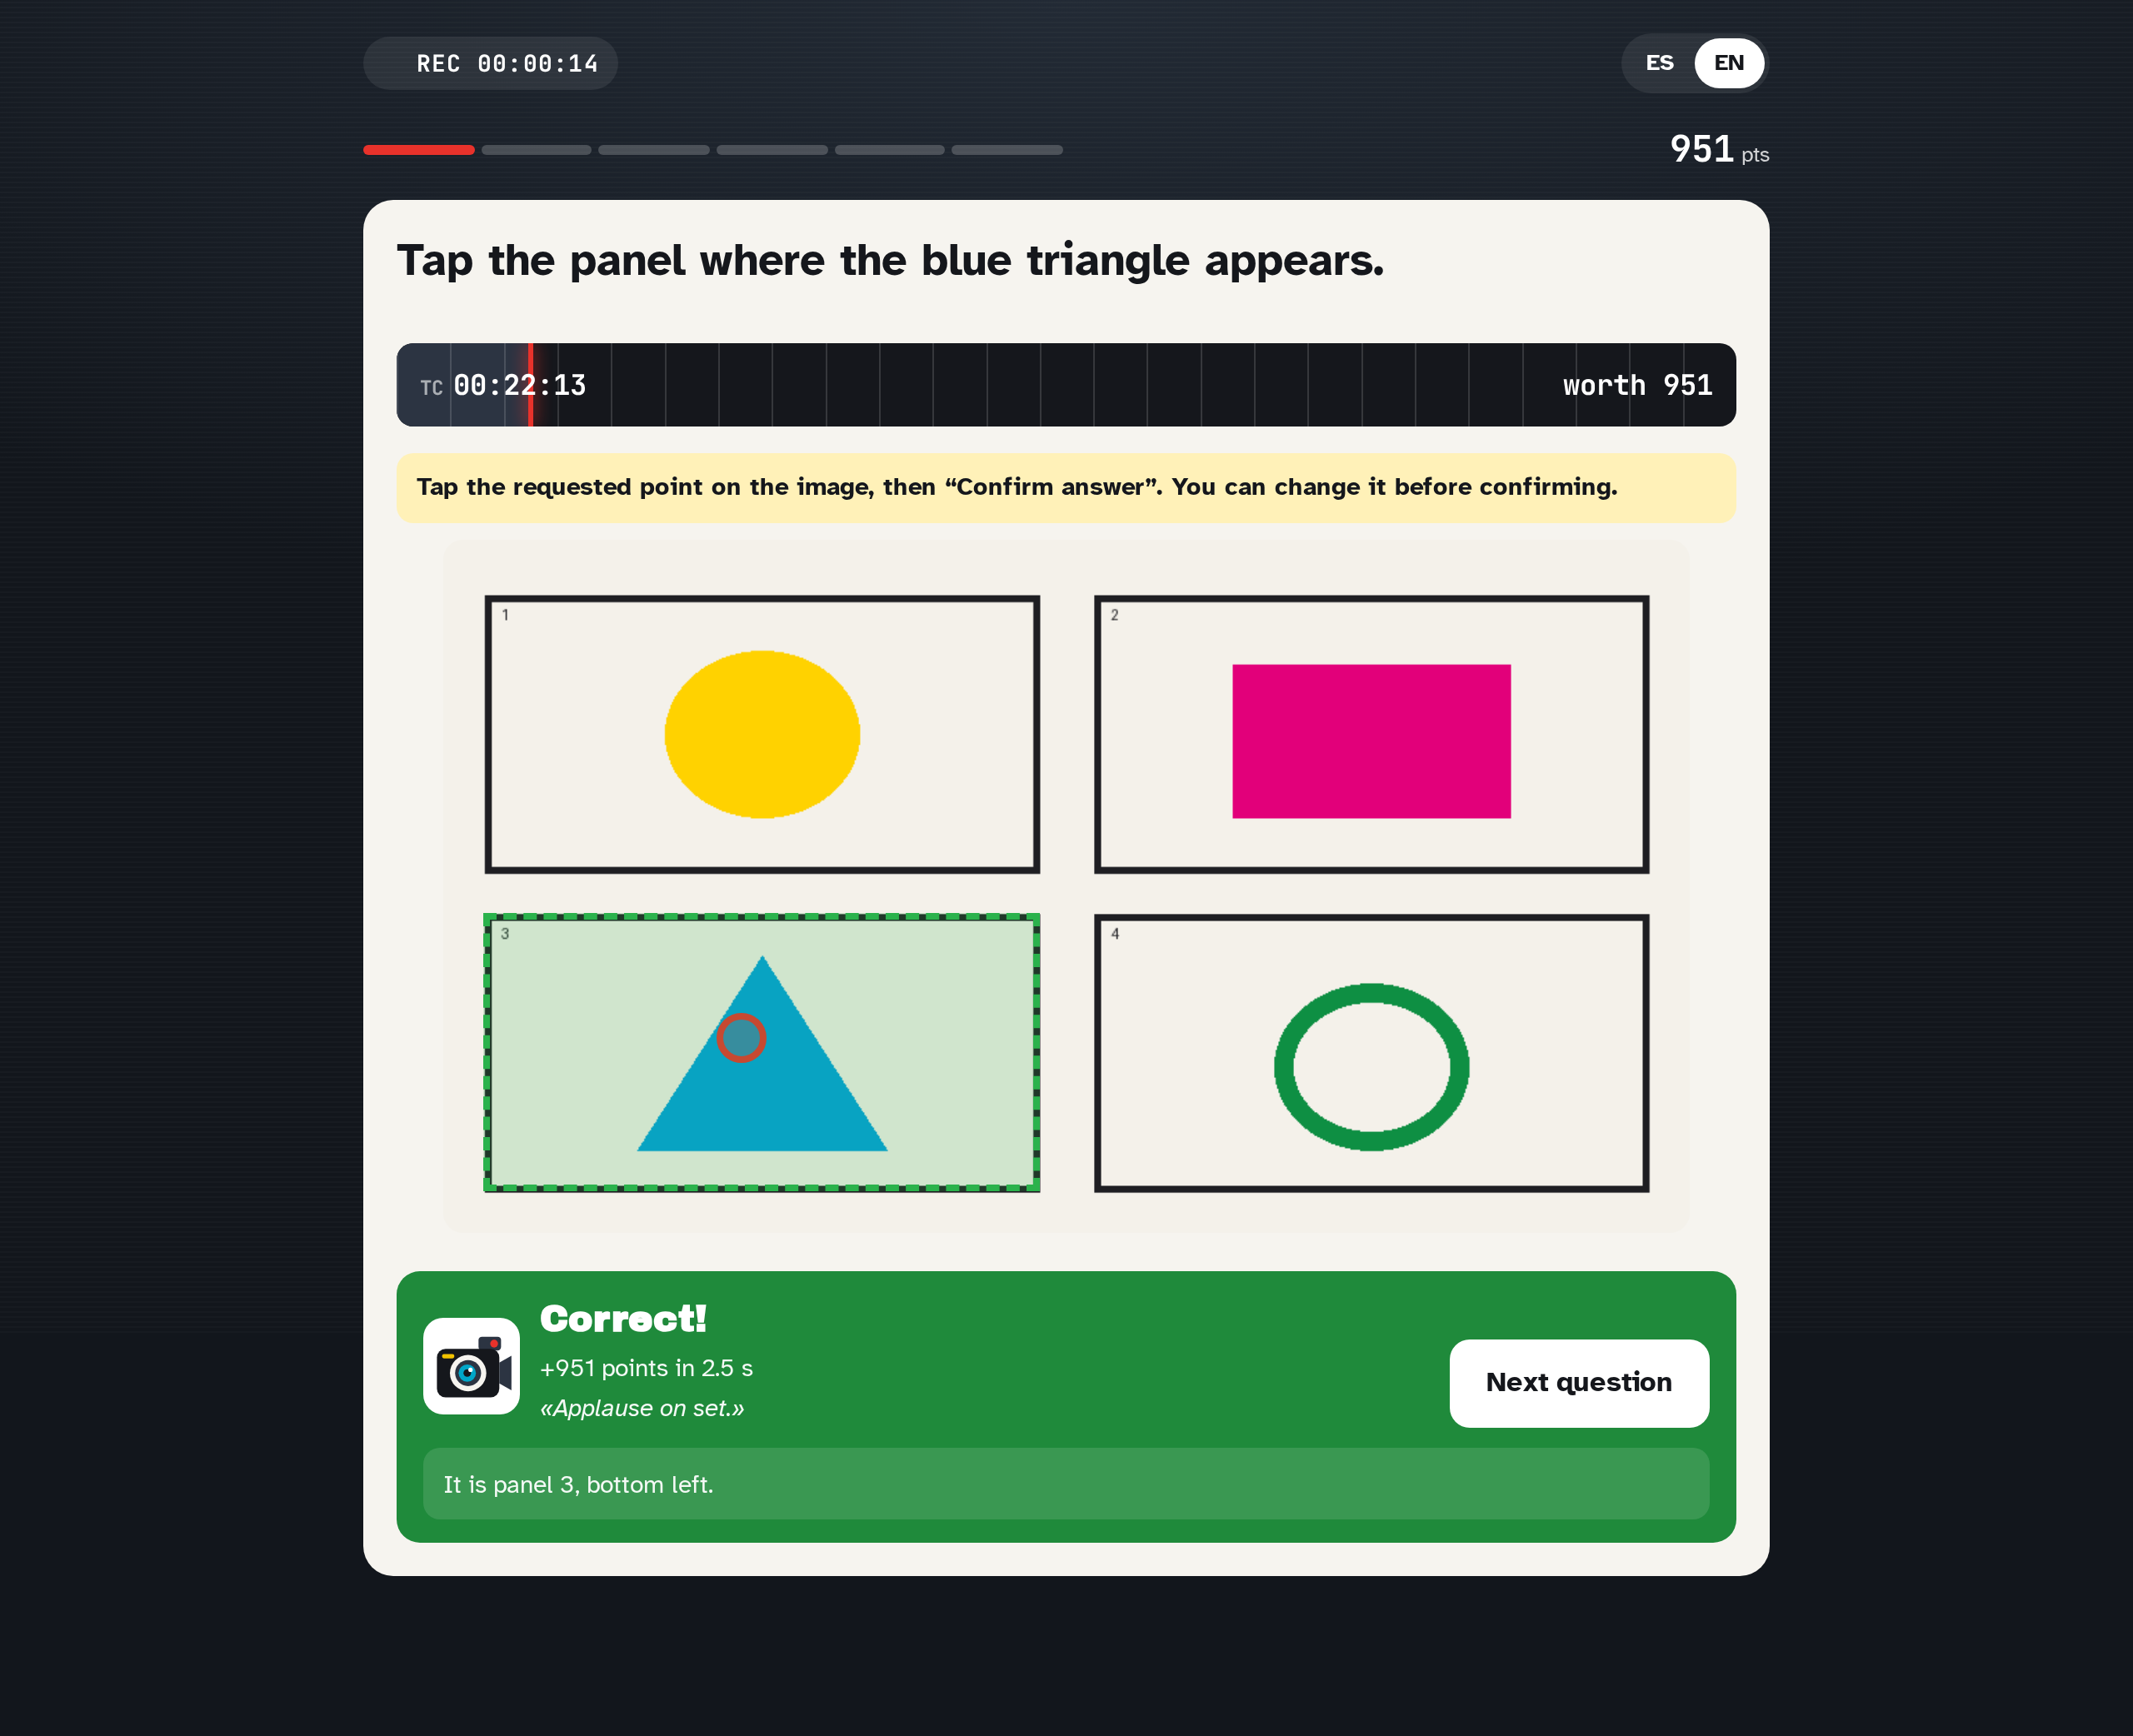
\includegraphics[width=\textwidth]{figures/10-floor-point-on-image.png}\\[1pt]{\small (a)}\\[4pt]
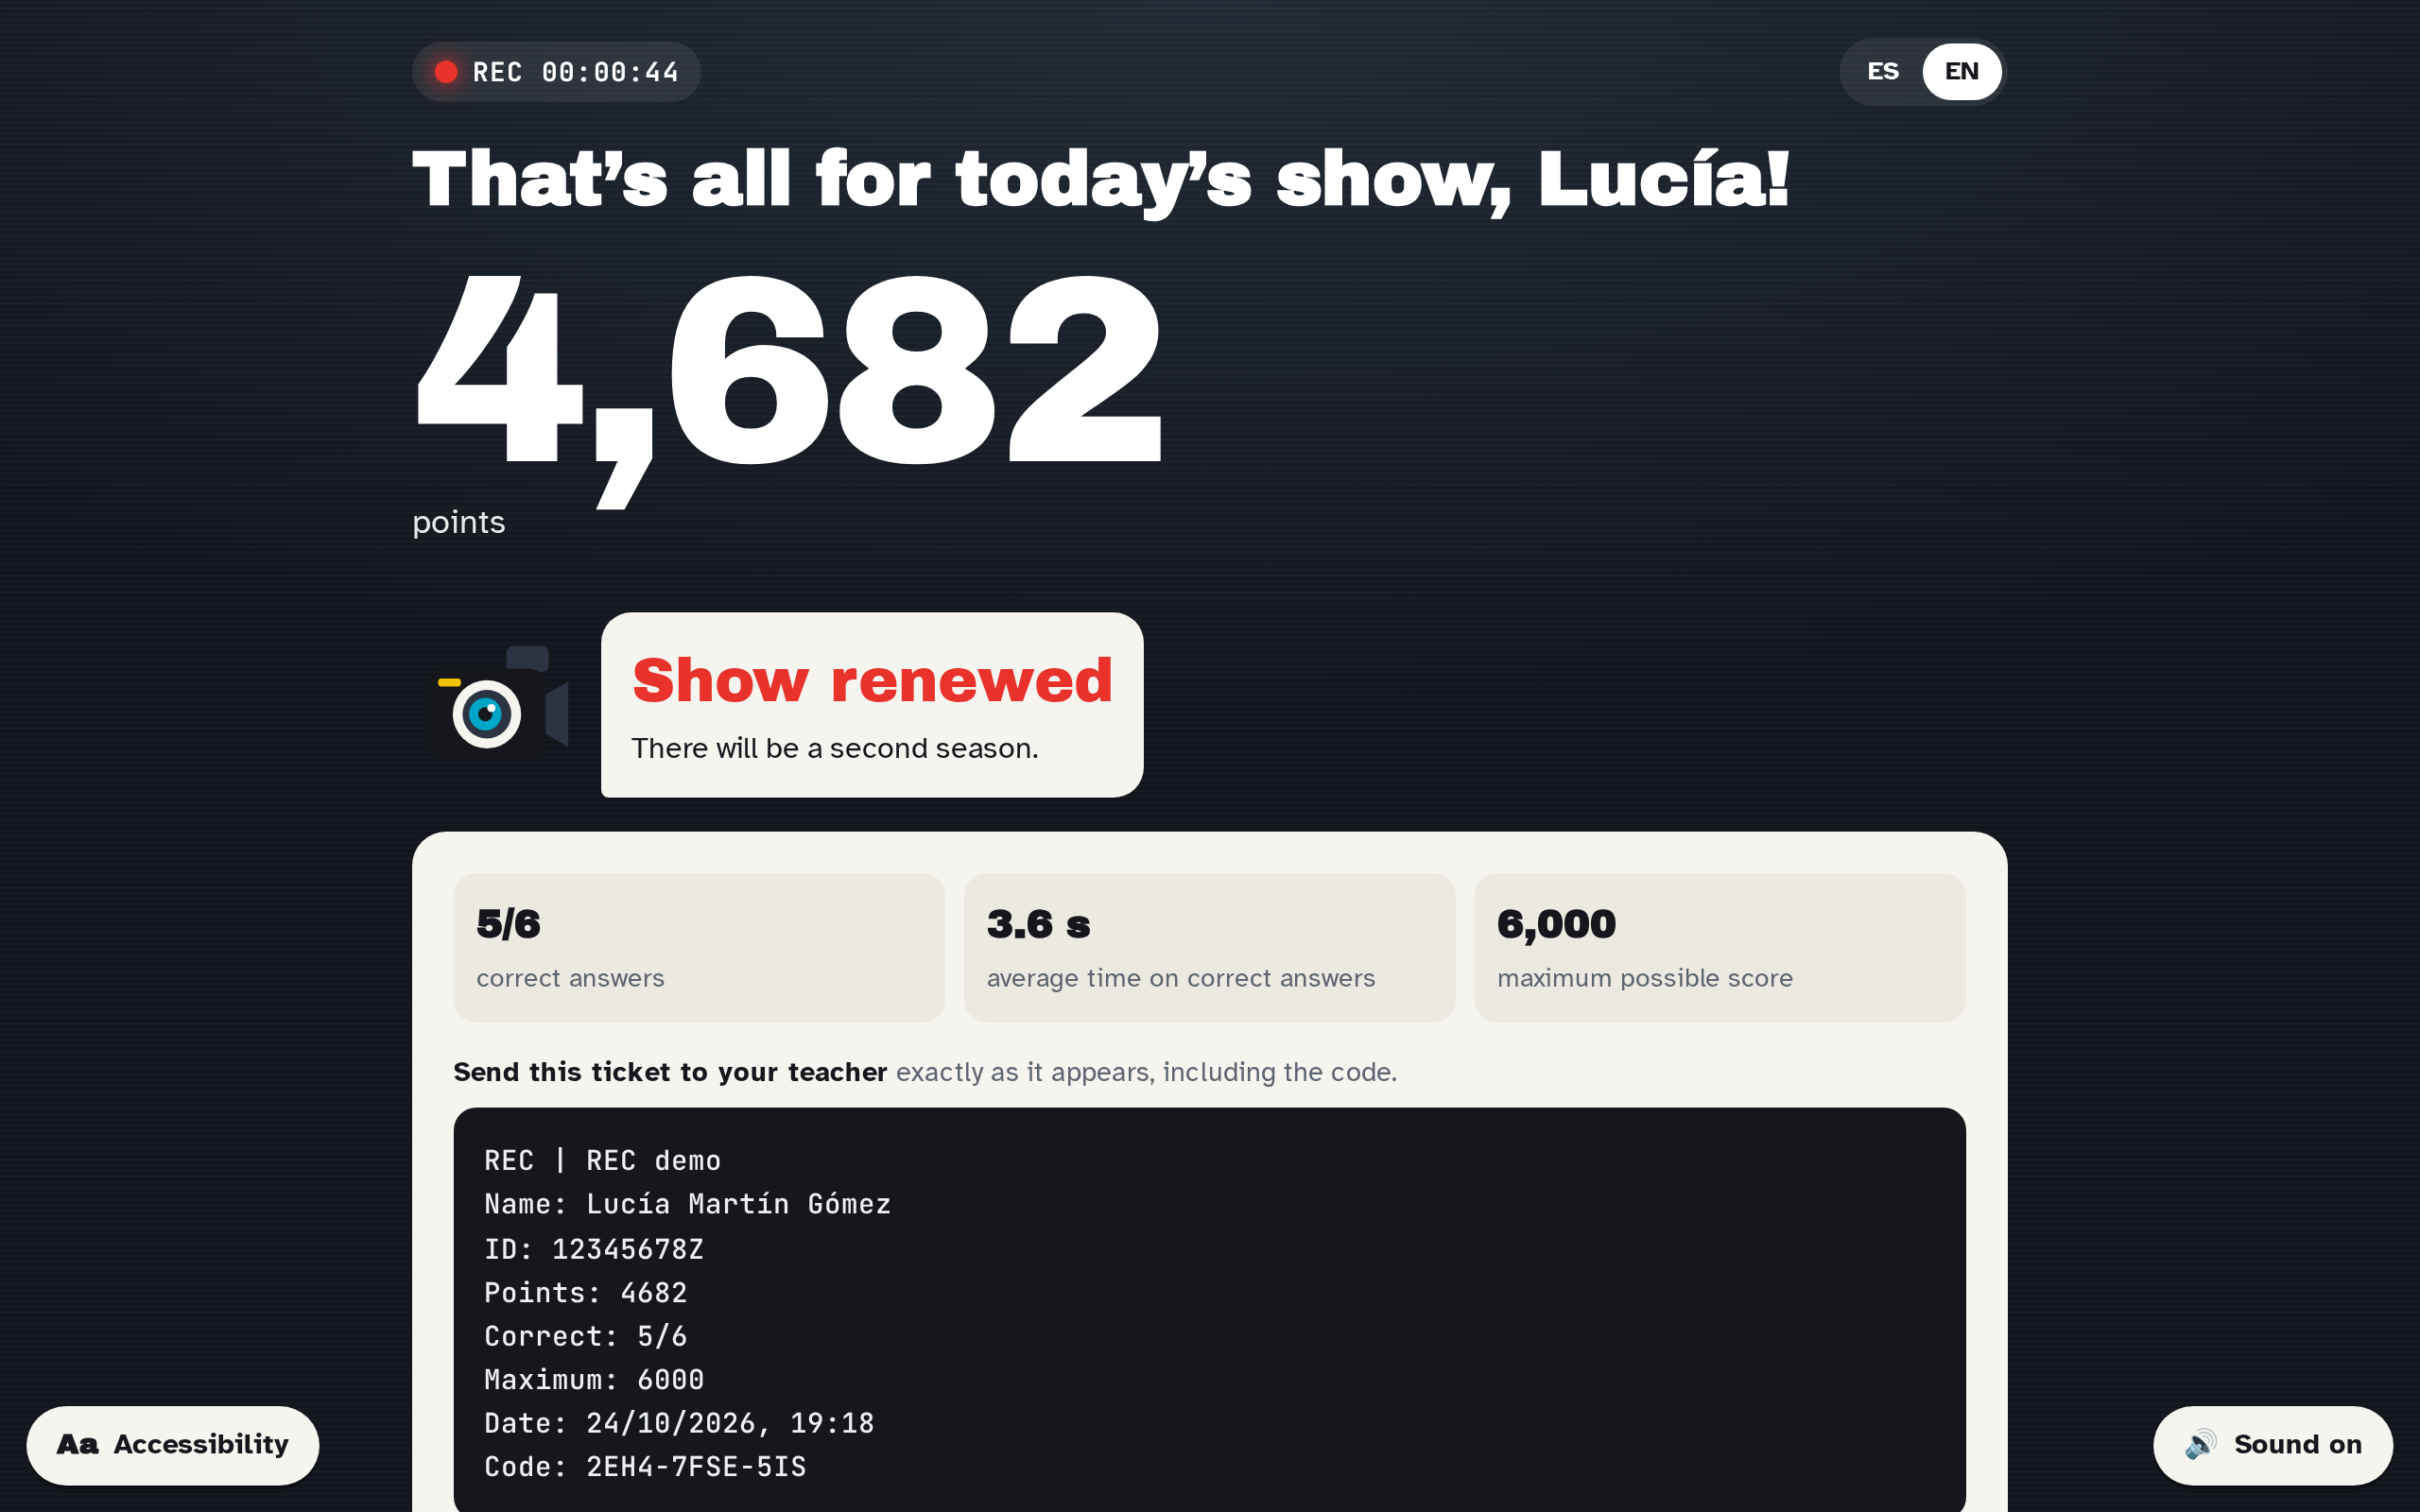
\includegraphics[width=\textwidth]{figures/11-floor-final-result.png}\\[1pt]{\small (c)}
\end{minipage}\hfill
\begin{minipage}[c]{0.36\textwidth}\centering
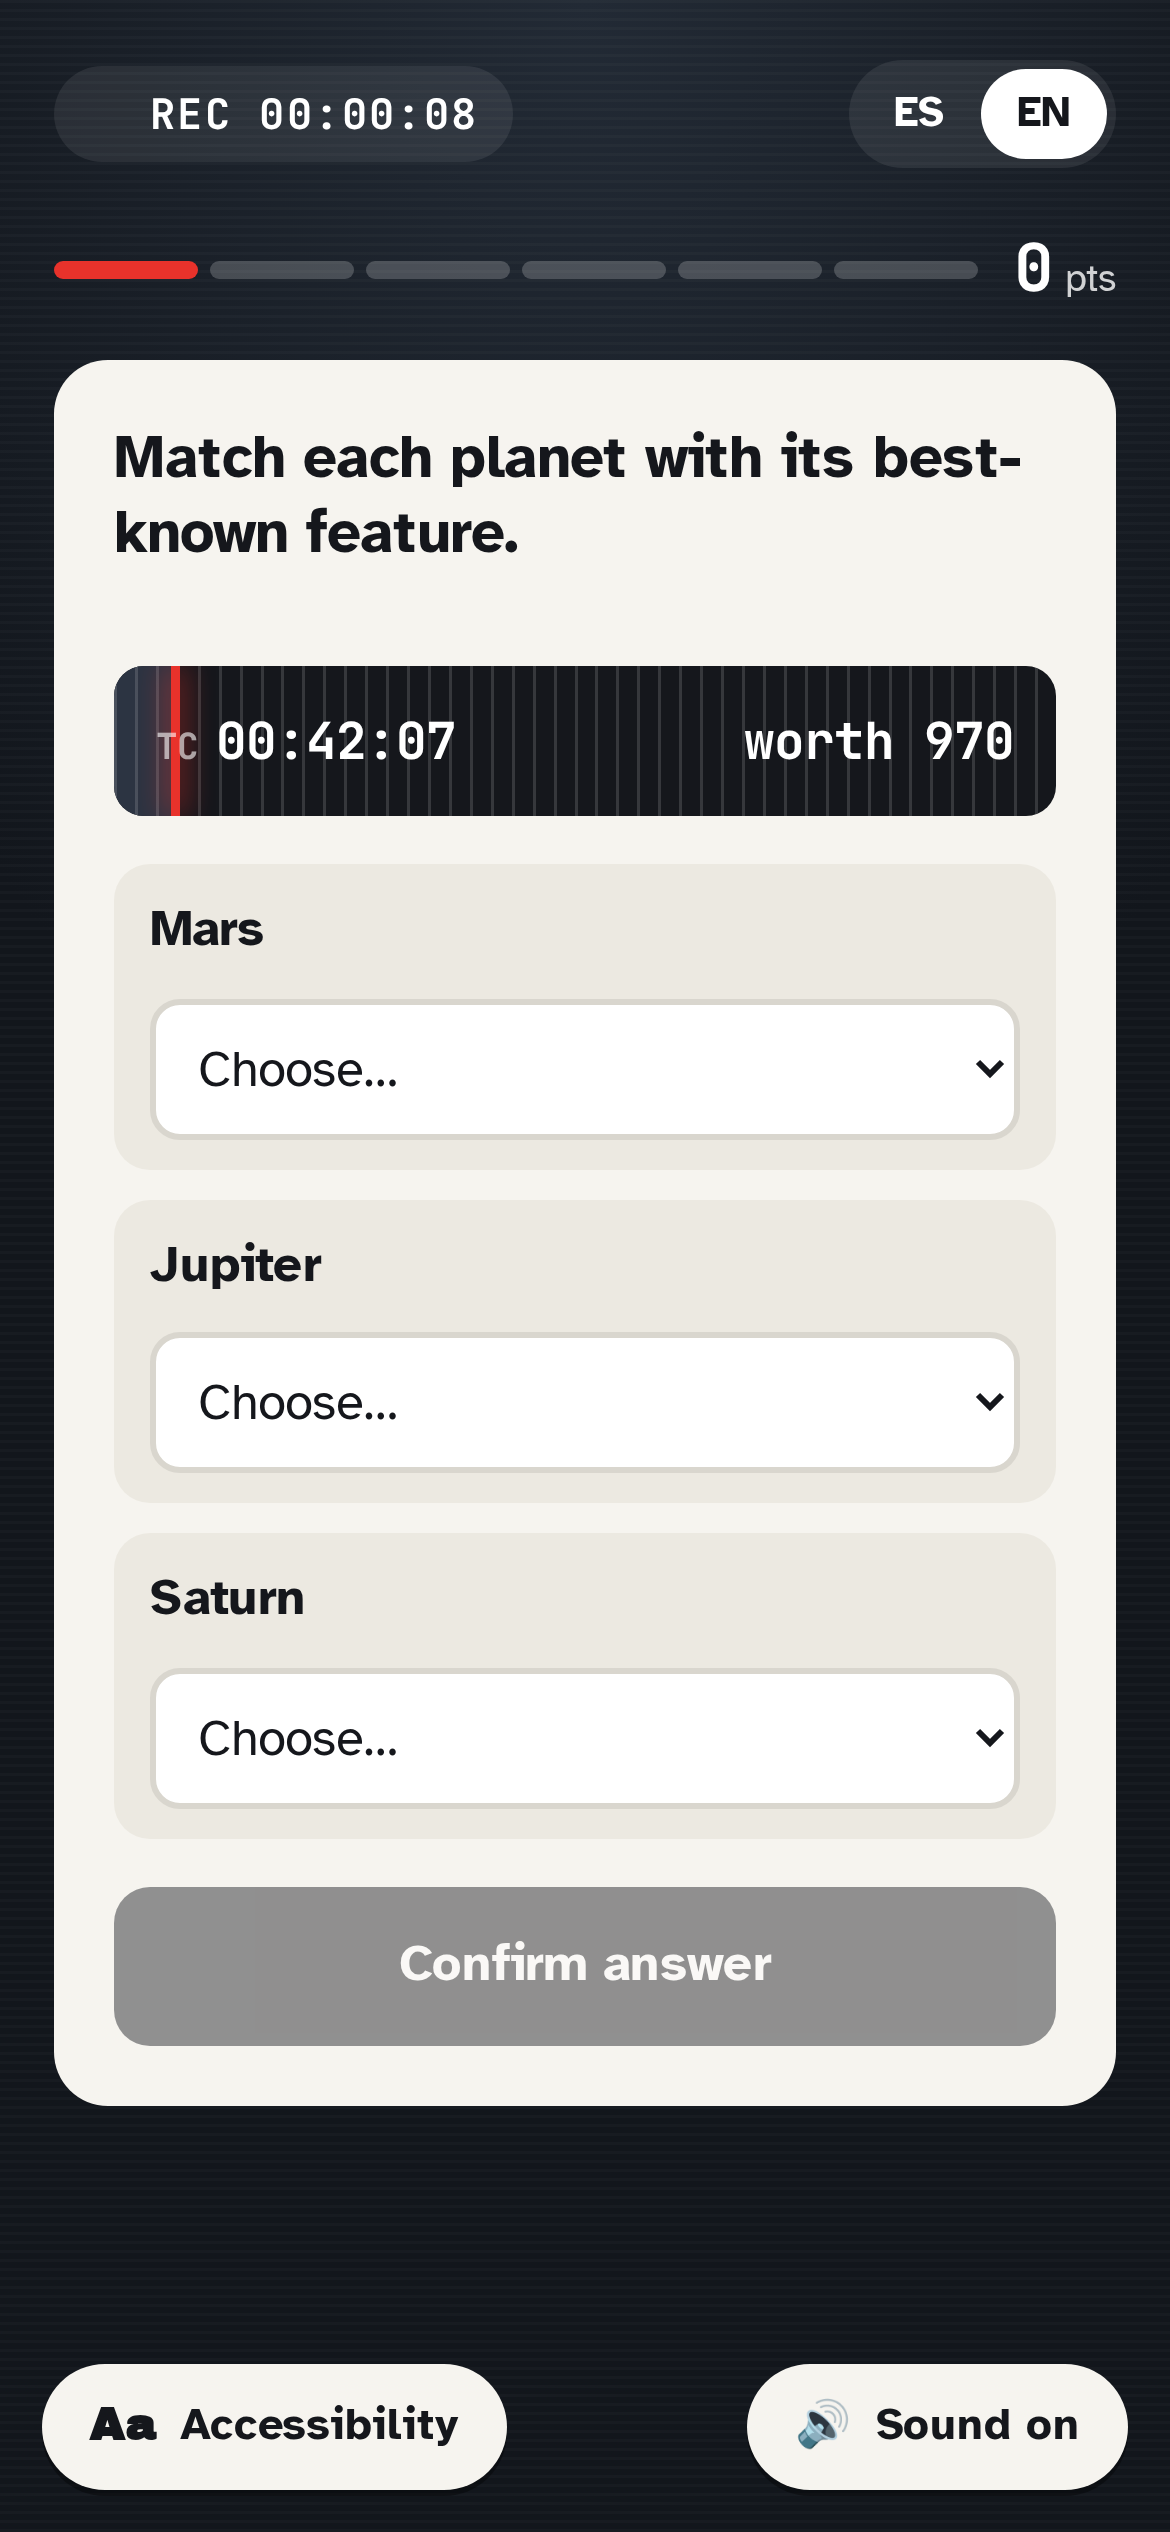
\includegraphics[width=\textwidth]{figures/16-floor-mobile-question.png}\\[1pt]{\small (b)}
\end{minipage}
\caption{The studio floor: (a)~a point-on-image question after a correct answer, with the points earned and the time used; (b)~a matching question on a phone; (c)~the end of the contest, with the ticket and its verification code. Students' data are fictitious.}
\label{fig:floor}
\end{figure}

\paragraph{Tickets} At the end, the student obtains a ticket with the score and a verification code computed from the contest, the student's identity and the result, and downloads it as a file of xAPI statements~\cite{xapi}, one per question, with the answer, its correctness, the time used, the time limit and the topic. When the teacher loads the tickets, the studio detects tickets that have been modified and duplicates. Because REC has no server, the code is computed in the student's browser: a student who recomputed it with the browser's developer tools would not be detected, and the same applies to the codes for extra time.

\paragraph{Ranking} From the tickets of a contest or section, the studio builds the ranking and assigns a bonus of questions counted as correct in the final exam, either by levels of the percentage of the maximum score or relative to the top scorer. The ranking can be published with or without names and downloaded as a spreadsheet.

\paragraph{Analysis} Each answer is classified by comparing its response time with the median for that question: correct and fast, correct and slow, wrong and fast, or wrong and slow (including time-outs). The \emph{speed and accuracy map} places each student by these two dimensions (Figure~\ref{fig:map}), and a question is flagged as a possible misconception when at least 30\% of the students answered it fast and wrong, in line with the finding that misconception-like answers tend to be given faster~\cite{heckler2015}. Because fast errors may also be guesses, and a confident error does not always reveal a misconception~\cite{hull2022}, the flags are presented as hypotheses for the teacher. The studio also reports the difficulty and discrimination of each question and mastery by topic; measures retention by comparing the answers in the sessions of a block with those in its global test; suggests ideas for the next class from fixed rules; projects the most-failed questions for a class review; and exports anonymised results as CSV or xAPI.

\begin{figure}[!htb]
\centering
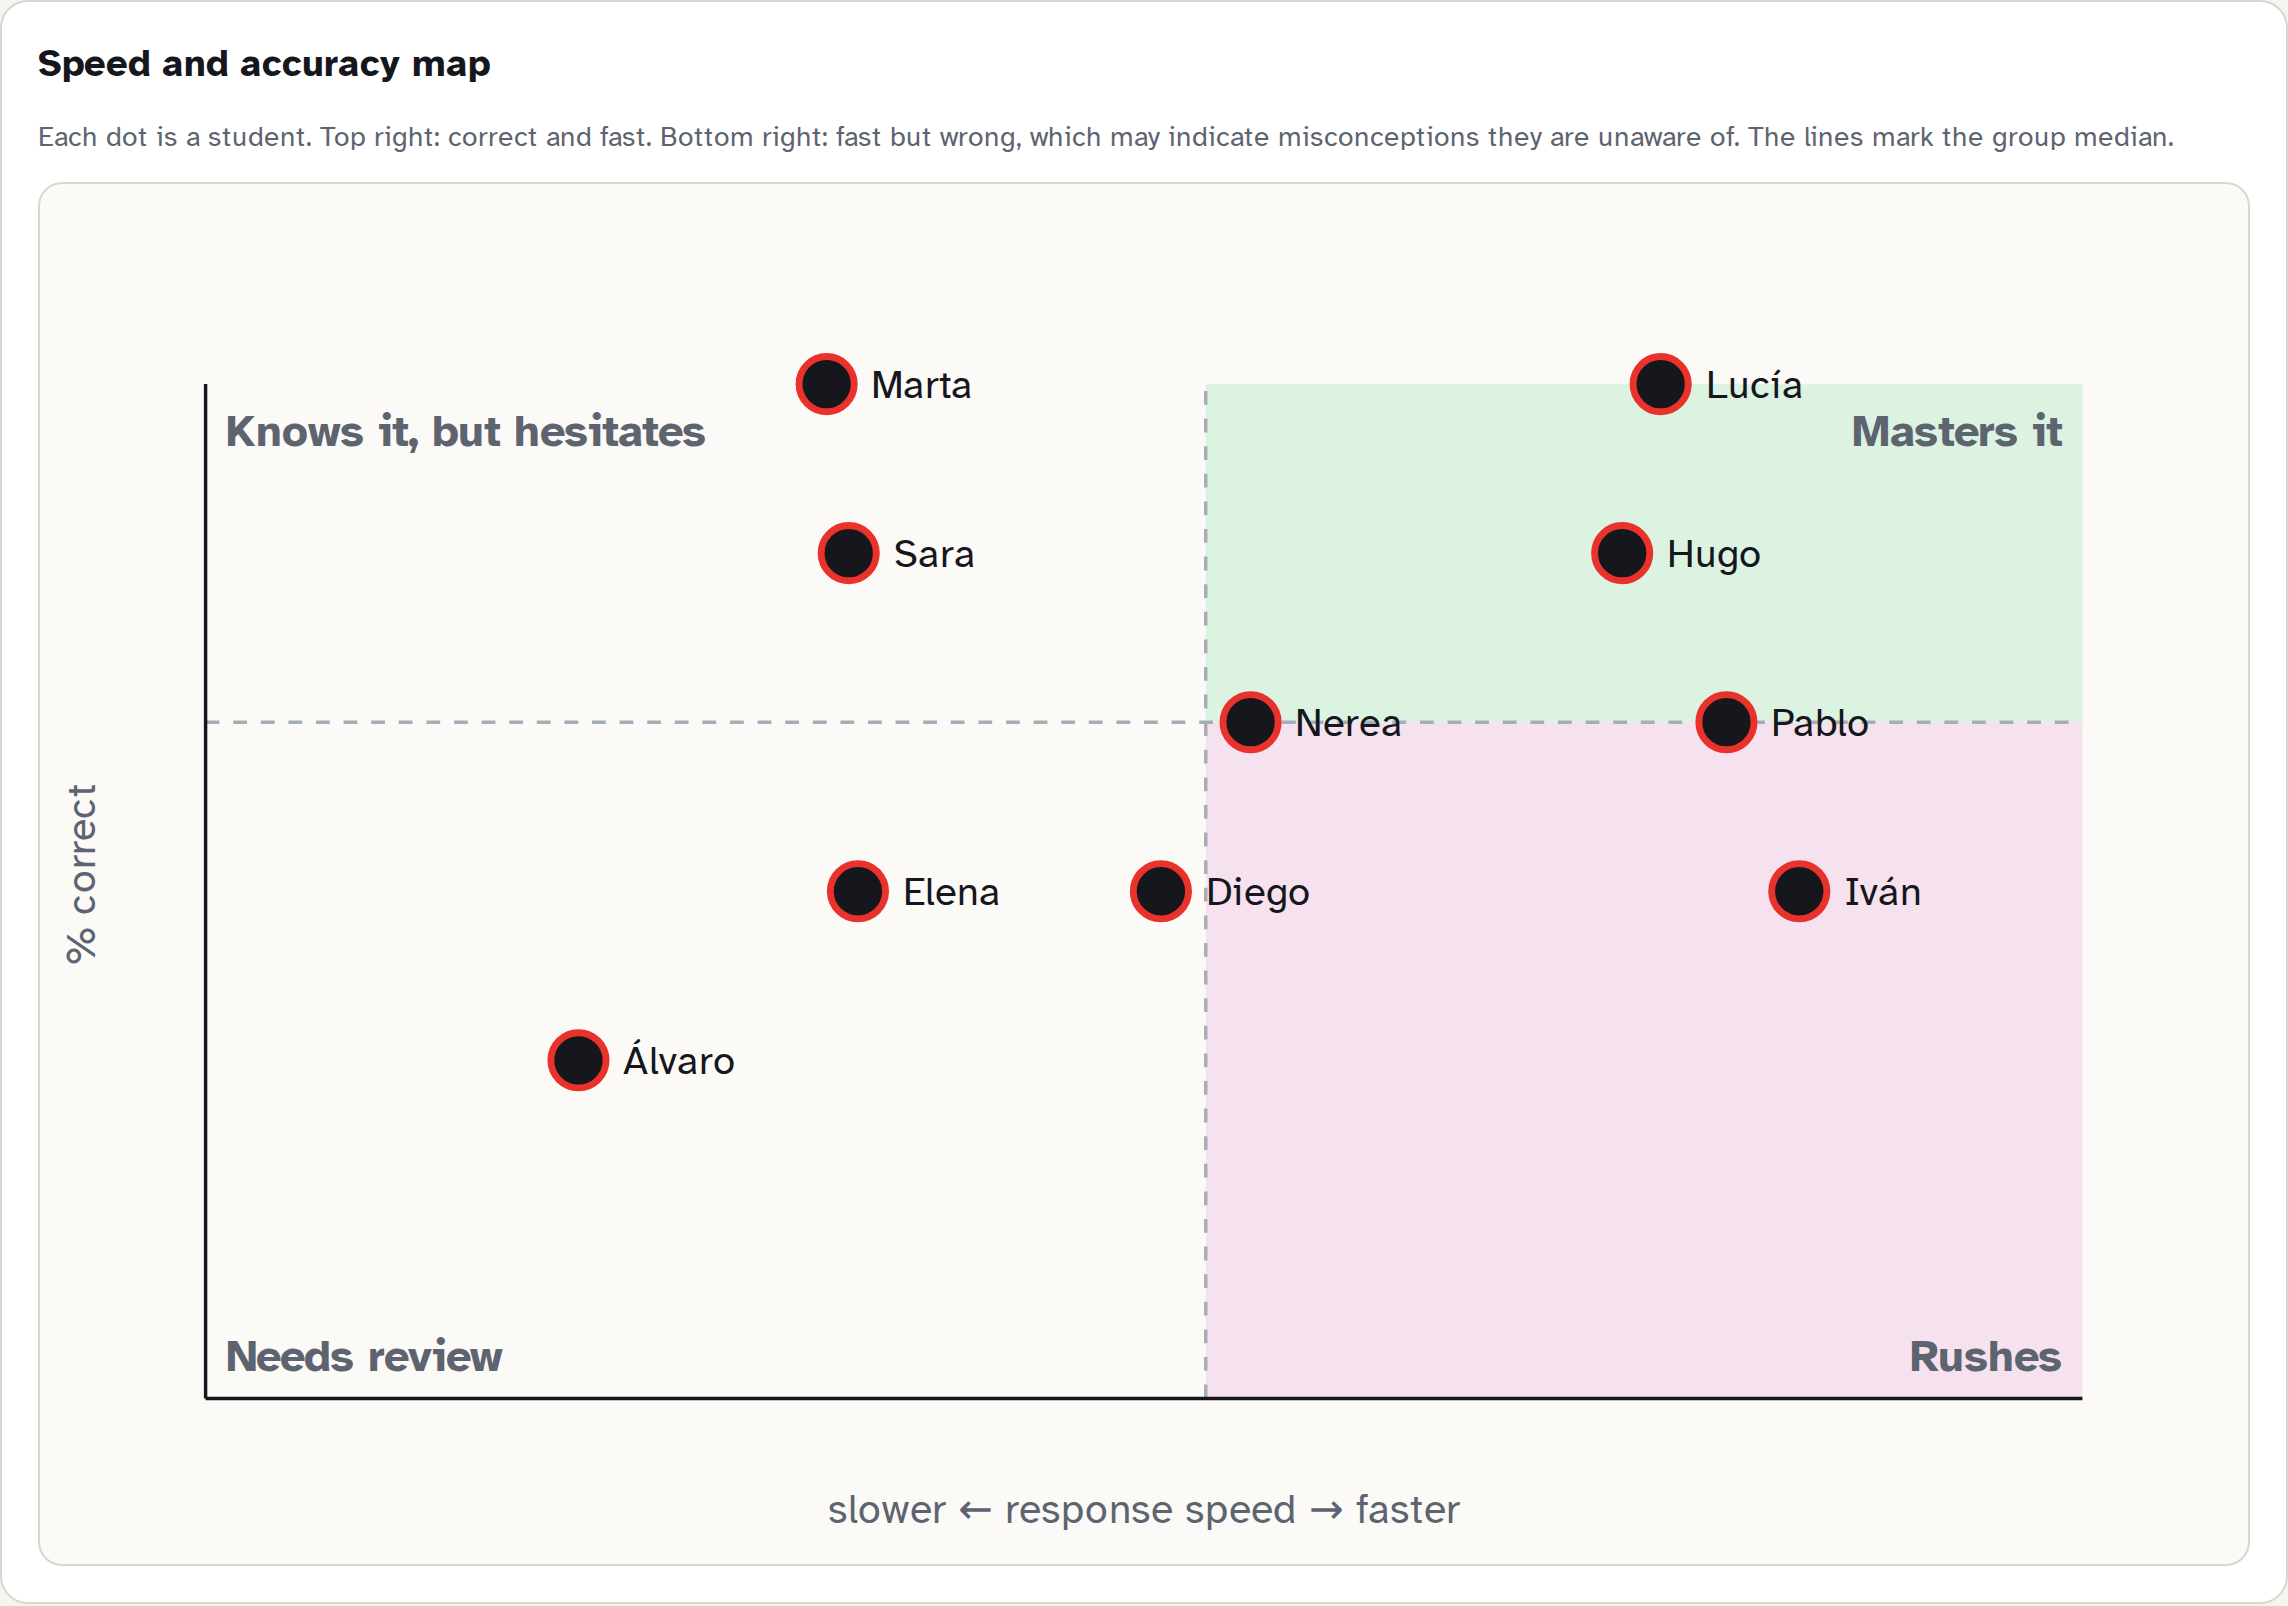
\includegraphics[width=0.8\textwidth]{figures/28-studio-speed-accuracy-map.png}
\caption{Speed and accuracy map of a contest. The dashed lines mark the group medians. Students' names are fictitious. \todo{Replace with anonymised real data after June?}}
\label{fig:map}
\end{figure}

%% ============================================================================
\section{Illustrative examples}
\label{sec:examples}

The two examples come from courses taught by the first author at the University of Cádiz in the second semester of the 2026/27 academic year, and show how the same tool adapts to two different uses. Students' data were anonymised before analysis \todo{reference to the university's consent}. In both courses, students played after the lecture, at the same time, on their own laptops, phones or tablets \todo{number of students per device type, if collected}, and submitted their tickets through the virtual campus. A screencast of the complete workflow is provided as supplementary material \todo{record}.

\paragraph{Graded continuous assessment} In \emph{Animación y Nuevas Tecnologías en Publicidad}, an elective course with \todo{N} students, the quizzes held after each lecture count towards continuous assessment, and the rankings award questions counted as correct in the final exam. A contest was created from scratch in the studio by importing the course's questions from Moodle XML, which took \todo{X} minutes from the import to the published package. After the session, loading the \todo{N} tickets and building the ranking took \todo{Y} minutes, compared with 15 to 30 minutes per quiz with the former spreadsheet. The bonus was assigned by levels of the percentage of the maximum score \todo{levels used}. The studio flagged \todo{question and concept} as a possible misconception, since \todo{p}\% of the students answered it fast and wrong; in the next class, \todo{what the teacher did}. \todo{Retention between the sessions of a block and its global test, if they are all run in REC.}

\paragraph{Diagnostic quizzes and attendance} In \emph{Fundamentos Técnicos en la Publicidad Digital}, with \todo{N} students, three ungraded contests were held before the corresponding topics were explained, to find out what students already knew and to record attendance; taking part added 0.1 points to the participation mark. \todo{Results: tickets received, tickets detected as modified or duplicated, questions flagged and how the lecture was adapted.}

%% ============================================================================
\section{Impact}
\label{sec:impact}

\paragraph{Daily practice} REC's main contribution to its users' practice is that it adapts to each course, as the two examples show. The same tool runs games with groups of about 150 students without per-player fees; gives the teacher feedback on what students understood after a lecture, or on what they knew before it; records attendance; and motivates students to attend and pay attention, since their answers determine how many questions they will have counted as correct in the final exam. It also removes the manual work of computing rankings in a spreadsheet, which took 15 to 30 minutes per quiz \todo{compare with the times measured in Section~\ref{sec:examples}}.

\paragraph{Personalised exams} REC completes a continuous-assessment workflow with Aspa, an offline tool by the same authors that generates paper exams personalised for each student~\cite{aspa}: the bonus of each student in REC becomes the number of questions omitted from their personalised exam and counted as correct. At present, the teacher chooses which questions are omitted for each student; a direct export from REC in the format of Aspa's class list is planned. \todo{Cite the published Aspa article instead of the software DOI, if available.}

\paragraph{Research} Because REC gives the teacher each student's answers and response times as xAPI statements~\cite{xapi,serrano2017}, without depending on a provider, it makes it possible to study, in ordinary courses, questions that are hard to address with commercial tools. These include whether a bonus in the final exam increases participation and attendance, for which the attendance recorded by the tickets can be compared with that of earlier years \todo{optional: one aggregate attendance rate (attendees/enrolled) per year, Moodle years vs 2026/27, descriptive only; otherwise leave as a research question}; whether misconceptions shared by a large part of the group, detected from fast and wrong answers, persist in the global tests; and how response time relates to accuracy in different subjects, extending studies conducted with exported Kahoot! data~\cite{liang2024}. \todo{Teaching-innovation project of the University of Cádiz for 2027/28, once awarded.}

\paragraph{Use} REC~1.0.0 was released in October 2026 and is in its first year of use. In the second semester of 2026/27 it was used in two courses with different purposes \todo{numbers of students, contests and tickets}. REC grew out of \emph{En el aire}\footnote{\url{https://github.com/lorenagmad/En-el-aire}}, a prototype built for a single course, and generalises it so that each teacher can create their own site from the kit; REC-FTPD\footnote{\url{https://github.com/lorenagmad/REC-FTPD}} is the instance for \emph{Fundamentos Técnicos en la Publicidad Digital}. REC will be presented in the teaching-innovation call of the University of Cádiz for 2027/28. It is distributed under the AGPL licence and is not used commercially.

%% ============================================================================
\section{Conclusions}
\label{sec:conclusions}

REC is a tool for gamifying quizzes that adapts to any course: the same tool supports graded continuous assessment, with rankings that reward students in the final exam, and ungraded diagnostic quizzes that also record attendance. It works with large groups without student accounts or a server of its own: questions are published only encrypted, and students' answers reach the teacher in a file, so that no external provider stores them. After each session, the studio analyses the answers, including their response times, offline, and helps the teacher act in the next class. Its limits are the price of this serverless design: the verification code detects edited tickets but cannot stop a student from recomputing it, and the game is not synchronised in real time; removing them would require the server that REC avoids. Future work includes importing questions from the formats of other tools and exporting the bonus of each student directly to the class list of Aspa.

\section*{Acknowledgements}
\label{sec:acknowledgements}

\todo{Optional.}

%% References
\begin{thebibliography}{00}
\small

\bibitem{wang2020} A.~I. Wang, R.~Tahir, The effect of using Kahoot! for learning -- A literature review, Computers \& Education 149 (2020) 103818. \url{https://doi.org/10.1016/j.compedu.2020.103818}

\bibitem{gutierrez2018} L.~Gutiérrez-Madroñal, J.~C. Collado Machuca, Cómo potenciar y evaluar de forma continua, la asistencia, los conocimientos y la participación activa del alumno en el aula a través de la gamificación [Fostering and continuously assessing students' attendance, knowledge and active participation in class through gamification], in: III Jornadas de Innovación Docente Universitaria UCA. Libro de Actas, Universidad de Cádiz, 2018, pp. 54--59. ISBN 978-84-09-04190-9 (in Spanish).

\bibitem{kahoot2019} Kahoot!, Plans and billing options for schools, help centre article (updated 25 November 2019), archived at \url{https://web.archive.org/web/20191213032024/https://support.kahoot.com/hc/en-us/articles/360008246494-Plans-and-billing-options-for-schools} (accessed 23 October 2026).

\bibitem{kahoot2021} Kahoot!, How many players can join a game?, help centre article (updated 27 February 2021), archived at \url{https://web.archive.org/web/20210302015423/https://support.kahoot.com/hc/en-us/articles/115003072287-How-many-players-can-join-a-game-} (accessed 23 October 2026).

\bibitem{kahoot} Kahoot!, \url{https://kahoot.com} and help centre \url{https://support.kahoot.com} (accessed 23 October 2026).

\bibitem{wayground} Wayground (formerly Quizizz), \url{https://wayground.com} and help centre \url{https://help.wayground.com} (accessed 23 October 2026).

\bibitem{socrative} Socrative, \url{https://www.socrative.com} and help centre \url{https://help.socrative.com} (accessed 23 October 2026).

\bibitem{blooket} Blooket, \url{https://www.blooket.com} and help centre \url{https://help.blooket.com} (accessed 23 October 2026).

\bibitem{gimkit} Gimkit, \url{https://www.gimkit.com} and help centre \url{https://help.gimkit.com} (accessed 23 October 2026).

\bibitem{mentimeter} Mentimeter, \url{https://www.mentimeter.com} and help centre \url{https://help.mentimeter.com} (accessed 23 October 2026).

\bibitem{moodlequiz} Moodle, Quiz activity documentation, \url{https://docs.moodle.org/en/Quiz_activity} (accessed 23 October 2026).

\bibitem{classquiz} ClassQuiz, \url{https://github.com/mawoka-myblock/ClassQuiz} (accessed 23 October 2026).

\bibitem{quizdock} QuizDock, \url{https://github.com/quizdock/quizdock} (accessed 23 October 2026).

\bibitem{heckler2015} A.~F. Heckler, T.~M. Scaife, Patterns of response times and response choices to science questions: The influence of relative processing time, Cognitive Science 39~(3) (2015) 496--537. \url{https://doi.org/10.1111/cogs.12166}

\bibitem{liang2024} Z.~Liang, More haste, less speed? Relationship between response time and response accuracy in gamified online quizzes in an undergraduate engineering course, Frontiers in Education 9 (2024) 1412954. \url{https://doi.org/10.3389/feduc.2024.1412954}

\bibitem{xapi} Advanced Distributed Learning Initiative, Experience API (xAPI) specification, version 1.0.3, \url{https://github.com/adlnet/xAPI-Spec} (accessed 23 October 2026).

\bibitem{rec} L.~Gutiérrez-Madroñal, R.~Baena-Pérez, J.~M. Mota-Macías, REC v1.0.0, Zenodo, 2026. \url{https://doi.org/10.5281/zenodo.23594648}

\bibitem{hull2022} M.~M. Hull, A.~Jansky, M.~Hopf, Does confidence in a wrong answer imply a misconception?, Physical Review Physics Education Research 18~(2) (2022) 020108. \url{https://doi.org/10.1103/PhysRevPhysEducRes.18.020108}

\bibitem{aspa} L.~Gutiérrez-Madroñal, R.~Baena-Pérez, J.~M. Mota-Macías, Aspa v1.0.0, Zenodo, 2026. \url{https://doi.org/10.5281/zenodo.23571011}

\bibitem{serrano2017} Á.~Serrano-Laguna, I.~Martínez-Ortiz, J.~Haag, D.~Regan, A.~Johnson, B.~Fernández-Manjón, Applying standards to systematize learning analytics in serious games, Computer Standards \& Interfaces 50 (2017) 116--123. \url{https://doi.org/10.1016/j.csi.2016.09.014}

\end{thebibliography}

\section*{Current executable software version}
\label{sec:execversion}

REC is a web application interpreted by the browser, so there is no compiled executable. The studio floor is available at \url{https://lorenagmad.github.io/REC/} and the studio at \url{https://lorenagmad.github.io/REC/studio.html}; the demonstration contest opens with the password \texttt{rec demo}.

\end{document}
\endinput
